\documentclass[9pt, xcolor={dvipsnames,svgnames,table}]{beamer}
\usepackage{eso-pic}
\beamertemplatenavigationsymbolsempty
\setbeamertemplate{footline}[frame number]

\newcommand\AtPagemyUpperLeft[1]{\AtPageLowerLeft{%
\put(\LenToUnit{0.85\paperwidth},\LenToUnit{0.9\paperheight}){#1}}}
\AddToShipoutPictureFG{
  \AtPagemyUpperLeft{{
\includegraphics[width=1.4cm,keepaspectratio]{MonashLogo.png}}}
}

\usepackage{bm}
\usepackage{amsmath}  
\usepackage{amsfonts} 
\usepackage{graphicx} 

\usepackage{mathtools}
\usepackage{algorithm}
\usepackage[noend]{algpseudocode}
\usepackage{float}
\usepackage[round]{natbib}
\usepackage{caption}


\newcommand{\F}{\mathcal{F}}
\renewcommand{\P}{\mathbb{P}}
\newcommand{\Q}{\mathbb{Q}}
\newcommand{\Real}{\mathbb R}
\renewcommand{\d}[1]{\ensuremath{\operatorname{d}\!{#1}}}


\title{Final Milestone MPhil: Novel Approaches on the Reconstruction of partially detected evolving Systems}
\author[Valentina Di Marco]{\textbf {Valentina Di Marco\\ \footnotesize Supervisors: Assoc. Professor Jonathan Keith (Monash University) and Distinguished Professor Kerrie Mengersen (Queensland University of Technology), \\ \footnotesize In collaboration with: Dr. Daniel Spring (University of Melbourne)}}

\date{\today}







\begin{document}

\begin{frame}
    \titlepage
\end{frame}

\begin{frame}
    \frametitle{Outline}
    \tableofcontents
\end{frame}



\section{Motivation}

\begin{frame}
\frametitle{What problem are we trying to solve}
We are considering
\begin{itemize}
\setlength\itemsep{1em}
    \item Systems that evolve in time and are only partially observed.
    \item Observations that are exact and arrive sequentially in time.
\end{itemize}
We will want to impute the missing observations for all elements created up to the current time.
\end{frame}


\begin{frame}
    \frametitle{What applications}
    The original motivation was to facilitate the analysis of the Red Imported Fire Ant (RIFA) invasion in Queensland.
    \begin{itemize}
        \item For detected nests, the location can be precisely determined, but there is an unknown number of undetected nests with unknown location. 
        \item To infer the current extent of the invasion, we impute plausible locations of undetected individuals. 
        \item These imputations are only informed guesses, and will require constant correction as new detections arrive. 
        \item In addition, new nests are constantly being produced as the state of the system is constantly evolving.
    \end{itemize}
    To handle this kind of problems we introduce a new Sequential Importance Sampling  strategy (`SIS with corrections'), which will allow us to make corrections each time new data is acquired.
\end{frame}


\begin{frame}
    \frametitle{Other applications}
    \begin{itemize}
    \setlength\itemsep{1em}
        \item Evolution of a species’ geographic range also for non invasive species.
        \item Bush fire \cite{}.
        \item Crime detection \cite{}.
        \item Infectious disease \cite{}.
    \end{itemize}
\end{frame}



\section{Existing methods}

\begin{frame}
    \frametitle{Existing methods}
    \begin{itemize}
        \setlength\itemsep{2em}
        \item In some cases, it is possible to obtain analytical solutions to compute the evolving sequence of posterior distributions, however, data is often complex and analytical solutions might be precluded.
        \item Sequential Monte Carlo methods are one of many solutions that can deal with this issue. If we have many samples from the posterior distribution we can approximate the posterior. 
        \item When it is impossible to obtain samples from these distributions directly we can use alternative Monte Carlo methods, like Importance Sampling.
        \item Importance Sampling however has the drawback that every time new data becomes available, one needs to recompute the importance weights over the entire state sequence. this means that as the time increases the computational complexity increases. Sequential importance sampling is a modification of Importance Sampling that can overcome this problem.
    \end{itemize}
\end{frame}

\section{Our method: SIS With Corrections}

\begin{frame}
    \frametitle{SIS With Corrections: the variables}
    Consider an $M$-dimensional system evolving in \textcolor{Fuchsia}{discrete time}.
    \begin{itemize}
        \item The \textcolor{PineGreen}{states of this system} at times $t = 1, \dots, T$ are represented by random vectors $\bm{x}^t = (x^t_1, \dots, x^t_M) \in \Real^M$ defined on a probability space $(\Omega, \F, \P)$. So, the \textcolor{PineGreen}{trajectory of the system} up to time $t$ is represented by a random matrix $\bm{X}^t = (\bm{x}^1, \ldots, \bm{x}^t)$. 
        \item Our \textcolor{PineGreen}{state of knowledge} regarding the trajectory of the system up to time $t$ is represented by a random binary matrix $\bm{b}^t = (b^t_{im}) \in 2^{t \times M}$, where $b^t_{im} = 1$ if the value of $x^i_m$ is known by time $t$, and $b^t_{im} = 0$ if the value of $x^i_m$ is still unknown at time $t$. We then define $\bm{B}^t = (\bm{b}^1,\ldots,\bm{b}^t)$.
        \item We define an \textcolor{PineGreen}{observation matrix} $\bm{z}^t = (z^t_{im})$, where $z^t_{im} = x^i_m$ if $b^t_{im} = 1$, and $z^t_{im} = -$ if $b^t_{im} = 0$. The symbol `$-$' is used to represent an unknown system coordinate. We also define $\bm{Z}^t = (\bm{z}^1,\ldots,\bm{z}^t)$.
    \end{itemize}
Observations are without error so are determined by $\bm{X}^t, \bm{B}^t$. We therefore define a function $\sigma_t: \Real^{t \times M} \times \left( \prod_{i=1}^t 2^{i \times M} \right) \rightarrow \prod_{i=1}^t (\Real \cup \{ - \})^{i \times M}$ such that $\bm{Z}^t = \sigma_t(\bm{X}^t, \bm{B}^t)$.
\end{frame}

\begin{frame}
    \frametitle{SIS With Corrections: at time $t=1$}
    At time $t=1$, our knowledge of the system is represented by a prior distribution with density $q(\bm{X}^1, \bm{B}^1)$ on $\Omega_1 = \Real^M \times 2^M$ and the posterior distribution after observing $\bm{Z}^1$ has a density on $\Omega_1' = \sigma^{-1}(\bm{Z}^1)$ given by:
    \begin{equation*}
        p(\bm{X}^1, \bm{B}^1 |\bm{Z}^1) = \frac{q(\bm{X}^1, \bm{B}^1)} {r(\bm{z}^1)} 
    \end{equation*}
    where
    \begin{align*}
        r(\bm{z}^1)  &= \int_{\Omega_1'} q(\bm{X}^1, \bm{B}^1) \prod_{ \{m \in \{1, \ldots, M \} : z^1_{1m} = - \} } \D x^1_m.
    \end{align*}
    Note that the preceding equation integrates over the elements of $\bm{X}^1$ that are not determined by $\bm{Z}^1$. Thus $r(\bm{z}^1)$ is the integral of $q(\bm{X}^1, \bm{B}^1)$ over $\Omega_1'$. 
\end{frame}

\begin{frame}
    \frametitle{SIS With Corrections: at time $t \geq 2$}
    Our knowledge of the trajectory of the system at time $t \geq 2$, before we acquire the next observation matrix $\bm{z}^t$, is represented by a prior distribution with density $q(\bm{X}^t, \bm{B}^t | \bm{Z}^{t-1})$ on the subspace $\Omega_t = \sigma^{-1}(\bm{Z}^{t-1}) \times \Real^M \times 2^{t \times M}$. After observing $\bm{z}^t$, certain pairs $(\bm{X}^t, \bm{B}^t)$ with non-zero prior density will be incompatible with the new observations, and the posterior density must therefore restrict $(\bm{X}^t, \bm{B}^t)$ to $\Omega_t' = \sigma^{-1}(\bm{Z}^t)$. The posterior density over $\Omega_t'$ must therefore be
    \begin{equation*}
        p(\bm{X}^t, \bm{B}^t |\bm{Z}^t) = \frac{q(\bm{X}^t, \bm{B}^t | \bm{Z}^{t-1})}{r(\bm{z}^t | \bm{Z}^{t-1})} 
    \end{equation*}
    where
    \begin{align*}
        r(\bm{z}^t | \bm{Z}^{t-1})  &= \int_{\Omega_t'} q(\bm{X}^t, \bm{B}^t | \bm{Z}^{t-1}) \prod_{ \{ i \leq t, m \in \{1, \ldots, M \} : z^t_{im} = - \} } \D x^i_m.
    \end{align*}
    Note that the preceding equation integrates over the elements of $\bm{X}^t$ that are not determined by $\bm{Z}^t$. Thus $r(\bm{z}^t | \bm{Z}^{t-1})$ is the integral of $q(\bm{X}^t, \bm{B}^t | \bm{Z}^{t-1})$ over $\Omega_t'$.
\end{frame}


\begin{frame}
    \frametitle{SIS With Corrections: Markovian Systems}
    We focus on \textcolor{Fuchsia}{Markovian systems}. 
   
    Let $f(\bm{x}^t | \bm{x}^{t-1})$ be the transitional density distribution characterising the system. 
   
    In general for $t \geq 2$ we have:
    \begin{align*}
        &(\bm{x}^t | \bm{x}^{t-1}) \sim f_t(\bm{x}^t | \bm{x}^{t-1})\\
        &(\bm{b}^t | \bm{x}^t, \bm{b}^{t-1}) \sim g_t(\bm{b}^t | \bm{x}^t, \bm{b}^{t-1})
    \end{align*}
    with densities of the initial states $f_1(\bm{x}^1)$ and $g_1(\bm{b}^1 | \bm{x}^1)$.
    The joint prior distribution for $(\bm{X}^t,\bm{B}^t)$ when $t=1$ is given by 
    \begin{equation*}
    q(\bm{X}^1,\bm{B}^1) = f(\bm{x}^1)g(\bm{b}^1 | \bm{x}^1)
    \end{equation*}
    and when $t \geq 2$: 
    \begin{eqnarray*}
        q(\bm{X}^t, \bm{B}^t | \bm{Z}^{t-1}) &=& f(\bm{x}^t | \bm{x}^{t-1}) g(\bm{b}^t | \bm{x}^t, \bm{b}^{t-1}) p(\bm{X}^{t-1}, \bm{B}^{t-1} | \bm{Z}^{t-1}) \\
        & = & \frac{f(\bm{x}^1)g(\bm{b}^1 | \bm{x}^1)}{r(\bm{z}^1)} \prod_{i=2}^{t-1} \frac{f(\bm{x}^i | \bm{x}^{i-1}) g(\bm{b}^i | \bm{x}^i, \bm{b}^{i-1})}{r(\bm{z}^i | \bm{Z}^{i-1})} \\
        & & \times f(\bm{x}^t | \bm{x}^{t-1}) g(\bm{b}^t | \bm{x}^t, \bm{b}^{t-1})
    \end{eqnarray*}
    on the space $\Omega_t$, and the joint posterior distribution on $\Omega_t'$ is given by:
    \begin{eqnarray*}
        p(\bm{X}^t, \bm{B}^t | \bm{Z}^t) 
        & = & \frac{f(\bm{x}^1)g(\bm{b}^1 | \bm{x}^1)}{r(\bm{z}^1)} \prod_{i=2}^t \frac{f(\bm{x}^i | \bm{x}^{i-1}) g(\bm{b}^i | \bm{x}^i , \bm{b}^{i-1})}{r(\bm{z}^t | \bm{Z}^{t-1})} 
    \end{eqnarray*}
\end{frame}


\begin{frame}
    \frametitle{SIS With Corrections: approximation of the posterior}
    We want to approximate the distribution $p(\bm{X}^{t}, \bm{B}^{t} | \bm{Z}^{t})$ by iterative sampling, and thus obtain Monte Carlo estimates of expectations of the form:
    \begin{align*}
        &E_{p} \Big[l(\bm{X}^{t}, \bm{B}^{t} ) \Big| \bm{Z}^{t} \Big] = \\
        &\int_{\Omega_t'} l(\bm{X}^{t}, \bm{B}^{t})\; p(\bm{X}^{t}, \bm{B}^{t} | \bm{Z}^{t})\; \prod_{ \{ i \leq t, m \in \{1, \ldots, M \} : z^t_{im} = - \} } \D x^i_m
    \end{align*}
    for functions $l: \Omega_t' \rightarrow \Real$. 
    \begin{itemize}
        \item We take a sequential importance sampling approach, at each iteration using a collection of weighted particles to approximate $p(\bm{X}^{t-1}, \bm{B}^{t-1} | \bm{Z}^{t-1})$.
        \item We evolve these particles under the model to create a new set of weighted particles representing the prior for iteration $t$, namely $q(\bm{X}^{t}, \bm{B}^{t} | \bm{Z}^{t-1})$.
        \item We then modify these particles to be consistent with the observations $\bm{Z}^{t}$, and adjust the weights to ensure the resulting weighted particles provide unbiased importance sampling estimates of an expectation $E_{p}[l(\bm{X}^{t}, \bm{B}^t) | \bm{Z}^t]$.
    \end{itemize}
\end{frame}

\begin{frame}
    \frametitle{SIS With Corrections: why we need corrections}
    Consider a particle $(\bm{X}^{t-1}_j,\bm{B}^{t-1}_j)$ constructed at time point $t$, for $j = 1, \ldots, n$, where $n$ is a fixed number of particles.
    \begin{itemize}
        \item We generate $\bm{x}^t_j$ for this particle by sampling from $f(\bm{x}^t | \bm{x}^{t-1}_j)$.
        \item Similarly, we generate $\bm{b}^{t}_j$ for this particle by sampling from $g(\bm{b}^{t} | \bm{x}^t_j, \bm{b}^{t-1}_j)$.
        \item The new matrix of observations $\bm{z}^{t}$ is typically inconsistent with a particle $(\bm{X}^{t}_j, \bm{B}^{t}_j)$ thus constructed, in two ways:
        \begin{itemize}
            \item the coordinates at which $\bm{b}^{t}_j$ contains a 0 may not correspond to the coordinates at which $\bm{z}^{t}$ contains a `$-$' and coordinates at which $\bm{b}^{t}_j$ contains a 1 may not correspond to an observation in $\bm{z}^{t}$.
            \item The observed values in $\bm{z}^{t}$ may differ from the corresponding coordinates of $\bm{X}^{t}_j$.
        \end{itemize}
    \end{itemize}
\end{frame}
    
\begin{frame}
    \frametitle{SIS With Corrections: deterministic corrections}
    We must therefore correct $\bm{X}^{t}_j$ and $\bm{b}^{t}_j$ in light of the new observations $\bm{z}^{t}$. 
    \begin{itemize}
        \item Replace $\bm{b}^{t}_j$ with the unique binary vector $(\bm{b}_j')^{t}$ that is consistent with $\bm{z}^{t}$.
        \item Replace the coordinates of $\bm{X}^{t}_j$ with the corresponding coordinates of $\bm{z}^{t}$ wherever $(\bm{b}_j')^{t}$ has a `1', thus generating a corrected term $\bm{(X')}^{t}_j$.
    \end{itemize}  
    The corrections made at time point $t$ will be carried forward into the particles used at all future times. 
    We use deterministic corrections in which the simulated pair $\bm{y}^{t} = (\bm{X}^{t}, \bm{B}^{t}) \in \Omega_t$ can be corrected in only one way to produce a new element $\bm{(y')}^{t} = (\bm{(X')}^t, \bm{(B')}^t) \in \Omega_t'$, that is
    \begin{equation*}
        \bm{(y')}^{t} = \rho(\bm{y}^{t},\bm{Z}^{t})
    \end{equation*}
    for some function $\rho$.
\end{frame}


\begin{frame}
    \frametitle{SIS With Corrections: Auxiliary variable}
    At each iteration, in order to simulate via a two-step process in which we generate a sample and then correct in light of data, we propose to use an auxiliary variable in the following manner.
    \begin{itemize}
        \item The auxiliary variable will be the yet to be corrected sample $\bm{y}^{t}$, which is an element of the space $\Omega_t$.
        \item We will use a projection map $\pi$ to relate the augmented space $\Omega^*_t = \Omega_t \times \Omega_t'$ containing elements of the form $(\bm{y}^{t}, \bm{(y')}^{t})$ to the corrected state space $\Omega_t'$ containing elements of the form $\bm{(y')}^{t}$.
        \item Our strategy is to define a probability density $p^*$ on $\Omega^*_t$, such that the marginal density of $p^*$ on $\Omega_t'$ is $p$.
        \item Similarly, we define a density $q^*$ on $\Omega^*_t$, such that the marginal density of $q^*$ on $\Omega_t$ is $q$.
        \item We then use a sequential importance sampling approach to re-weight a sample of particles used for Monte Carlo estimation with respect to $q^*$, so that they can be used for Monte Carlo estimation with respect to $p^*$.
    \end{itemize}
\end{frame}


\begin{frame}
    \frametitle{SIS With Corrections: $p^*$ and $q^*$}
    A key identity underlying this strategy is the following.
    \begin{equation*}
        E_{p}[l(\bm{(y')}^{t})]  =  E_{p^*}[l(\pi (\bm{y}^{t}, \bm{(y')}^{t})]
    \end{equation*}
    In this equation, the expectation on the left is over $\Omega_t'$, whereas the expectation on the right is over $\Omega_t^*$.
    
    Here we are here interested in a deterministic correction, so we define both $p^*$ and $q^*$ on a subspace of $\Omega_t^*$ consisting of points of the form $(\bm{y}^{t}, \rho(\bm{y}^{t}, \bm{Z}^{t}))$. The densities $p^*$ and $q^*$ are defined with respect to a reference measure on this subspace, constructed with the aid of Rohlin's disintegration theorem (\cite{Rohlin}).
    
    Since $\bm{y}^{t}$ determines $\bm{(y')}^{t}$, but the reverse is not necessarily true, the new densities are of the form:
    \begin{align*}
        q^*(\bm{y}^{t},\bm{(y')}^{t}) &= q(\bm{y}^{t} | \bm{Z}^{t-1}), \mbox{ and } \\
        p^*(\bm{y}^{t},\bm{(y')}^{t}) &= u(\bm{y}^{t} | \bm{(y')}^{t}) p(\bm{(y')}^{t} | \bm{Z}^{t})
    \end{align*}
    where $\bm{(y')}^{t} = \rho(\bm{y}^{t}, \bm{Z}^{t})$. Here $u$ is the density of some distribution over the set $F(\bm{(y')}^{t}) = \{ \bm{y} \in \Omega^t  :  \rho(\bm{y}, \bm{Z}^{t}) = \bm{(y')}^{t}\}$.
\end{frame}

\begin{frame}
    \frametitle{SIS With Corrections: the distribution $u$}
    The set $F(\bm{(y')}^{t})$ contains all elements of $\Omega^t$ that can be corrected to $\bm{(y')}^{t}$. It can be characterised as the set of elements of the form $(\bm{X}^{t},\bm{B}^{t}) \in \Omega^t$ such that:
    \begin{enumerate}
        \item $\bm{b}^{j} = (\bm{b}')^{j}$ for all $j < t$,
        \item $b_{im}^{t} = (b_{im}')^t$ whenever $(b_{im}')^t = (b_{im}')^{t-1}$, otherwise $b_{im}^{t} \in \{ 0, 1 \}$, and
        \item $x_{m}^{i} = (x_{m}')^{i}$ whenever $(b_{im}')^t = (b_{im}')^{t-1}$, otherwise $x_{m}^{i} \in \Real$.
    \end{enumerate}
    Thus $F(\bm{(y')}^{t})$ is isomorphic to $\Real^k \times 2^k$, where $k$ is the number of newly observed coordinates.
    
    \begin{itemize}
        \item The density $u$ must ensure $\esssupp(p^*) \subseteq \esssupp(q^*)$, (a requirement for valid importance sampling (\cite{Geweke})).
        \item Here we consider $u$ to be the uniform density on a bounded (to ensure integrability) subset of $F(\bm{(y')}^{t})$.
        \item If the bounded set is a hyper-rectangle, with each undetermined coordinate of $\bm{y}^{t}$ bounded independently of the others, the normalising constant of $u$ depends on $k$, but is otherwise independent of $\bm{(y')}^{t}$.
        \item If $\bm{y}^t$ is outside this hyper-rectangle, then $u(\bm{y}^t) = 0$, and this will result in zero-weighted particle. However, bounds can be set large enough that zero-weighted particles occur only infrequently.
    \end{itemize}
       
\end{frame}


\begin{frame}
    \frametitle{SIS With Corrections: The weights}
    Applying importance sampling on the probability space $\Omega^*$ we have
    \begin{align*}
        E_{p^*}[l(\pi (\bm{(y')}^{t}, \bm{y}^{t})] 
        \approx \sum_{j=1}^n  w^{t}_j l((\bm{y}'_j)^{t})
    \end{align*}
    where the weights are given by:
    \begin{eqnarray*}
        w^{t}_j &\propto& \frac{p^*(\bm{y}_j^{t}, (\bm{y}_j')^{t} | \bm{Z}^{t})} {q^*(\bm{y}_j^{t}, (\bm{y}_j')^{t} |\bm{Z}^{t-1})} \\
        &=& \frac{u(\bm{y}_j^{t} | (\bm{y}_j')^{t}, \bm{Z}^{t})}{r(\bm{z}^{t} | \bm{Z}^{t-1})} \frac{q((\bm{y}_j')^{t} | \bm{Z}^{t-1})}{q(\bm{y}_j^{t} | \bm{Z}^{t-1})} \\
        & \propto & u(\bm{y}_j^{t} | (\bm{y}_j')^{t}, \bm{Z}^{t}) \prod_{i=1}^{t} w^{t}_{ij}
    \end{eqnarray*}
    with
    \begin{eqnarray*}
        w^{t}_{1j} &=& \frac{f((\bm{x}_j')^1)}{f(\bm{x}_j^1)} \frac{g((\bm{b}_j')^1 | (\bm{x}_j')^1)}{g(\bm{b}_j^1 | \bm{x}_j^1)}
    \end{eqnarray*}
    and
    \begin{eqnarray*}
        w^{t}_{ij} &=& \frac{f((\bm{x}_j')^i | (\bm{x}_j')^{i-1})}{f(\bm{x}_j^i | \bm{x}_j^{i-1})} \frac{g((\bm{b}_j')^i | (\bm{x}_j')^i, \bm{b}_j^{i-1})}{g(\bm{b}_j^i | \bm{x}_j^i, \bm{b}_j^{i-1})}
    \end{eqnarray*}
\end{frame}


\begin{frame}
    \frametitle{Our method: The weights}
    for $i \geq 2$.
    Note the terms $u$ and $r$ are the same for all particles, and can be disregarded, since it will cancel after normalising the weights across particles. Note also that $(\bm{b}_j')^i$ differs from $\bm{b}_j^i$ only for $i = t$, since the older observations $\bm{z}^{i}$ have already fully determined $\bm{b}_j^i$ for $i < t$. 

    Therefore the normalised weights become:
    \begin{eqnarray*}
        w^{t}_j &=& \frac{\prod_{i=1}^t w^{t}_{ij}}{\sum_{j=1}^n \prod_{i=1}^t w^{t}_{ij}}.
    \end{eqnarray*}
    were
    \begin{equation*}
        w^{t}_{ij} = \frac{f((\bm{x}'_j)^i | (\bm{x}'_j)^{i-1})}{f(\bm{x}^i_j | \bm{x}^{i-1}_j)} 
    \end{equation*}
    for $i = 1 \dots, t-1$ and since the final $g$ term will not cancel
        \begin{eqnarray*}
            w^{t}_{tj} &=& \frac{f((\bm{x}_j')^t | (\bm{x}_j')^{t-1})}{f(\bm{x}_j^t | \bm{x}_j^{t-1})} \frac{g((\bm{b}_j')^t | \bm{b}_j^{t-1})}{g(\bm{b}_j^t | \bm{b}_j^{t-1})}.
        \end{eqnarray*}


\end{frame}



\section{Application: A simple AR(1) Model}

\begin{frame}
    \frametitle{Application to an AR(1) Model}
    \begin{itemize}
    \setlength\itemsep{2em}
        \item This new method has been applied to a Gaussian, linear and stationary AR(1) model with missing observations
        \item The observations were simulated from the model.
        \item For every particle $i$, the unnormalised weights at time $t$ for $b' \in \{0,1\}$ and $b \in \{0,1\}$ are calculated with the following formula
        \end{itemize}
    \begin{align*} \label{eq:2}
        &\frac{q(\bm{(X')}^{t} | \bm{Z}^{t-1}) }{q(\bm{X}^{t} | \bm{Z}^{t-1})} =
        \frac{\bigg \{ \prod_{s=2}^{t}  \frac{1}{\sqrt{2 \pi \sigma^{2}}} \exp \bigg [ { - \frac{1}{2 \sigma^{2}} }  (x'_s - \varphi x'_{s-1})^{2} \bigg ] \bigg \} }{\bigg \{ \prod_{s=2}^{t}  \frac{1}{\sqrt{2 \pi \sigma^{2}}} \exp \bigg [ { - \frac{1}{2 \sigma^{2}} }  (x_s - \varphi x_{s-1})^{2} \bigg ] \bigg \} } \nonumber, \\
        &\frac{p^{b'_t} (1 - p)^{1-b'_t}  }{ p^{b_t} (1 - p)^{1-b_t} }
    \end{align*}
    where the primed are the corrected terms.
\end{frame}


\begin{frame}
    \frametitle{The Analytical Solutions}
    \begin{itemize}
        \item In the AR(1) model with missing values, we use the last and the next existing observation and the definition of the model to evaluate analytically the missing data.
        \item These analytical estimations will be used as gold standard and compared to the results we get with `SIS with corrections'.
        \begin{align*}
            p(x_t | x_{\tau-1}, x_{m}) &= \mathcal{N} \Bigg(\frac{\varphi^{m-t} \sum_{i=0}^{t-\tau} \varphi^{2i} x_{m} + \varphi^{t-\tau+1} \sum_{i=0}^{m-t-1} \varphi^{2i} x_{\tau-1}}{\sum_{i=0}^{m-\tau} \varphi^{2i}}, \\
        & \frac{\sigma^2_\eta \sum_{i=0}^{m-t-1} \varphi^{2i} \sum_{i=0}^{t-\tau} \varphi^{2i}}{\sum_{i=0}^{m-\tau} \varphi^{2i}} \Bigg).
        \end{align*}
        Where $\tau-1$ is the index of the last observation before the block of missing values and $m$ is the fist observation after the block of missing values and $t = \tau, \dots, m-1$.
    \end{itemize}
\end{frame}

\begin{frame}
\frametitle{Simulations compared with gold standard for an AR(1) model}
\begin{figure}
%\begin{minipage}{1\textwidth}
%\centering
    \captionsetup{font=footnotesize}
    \subfloat{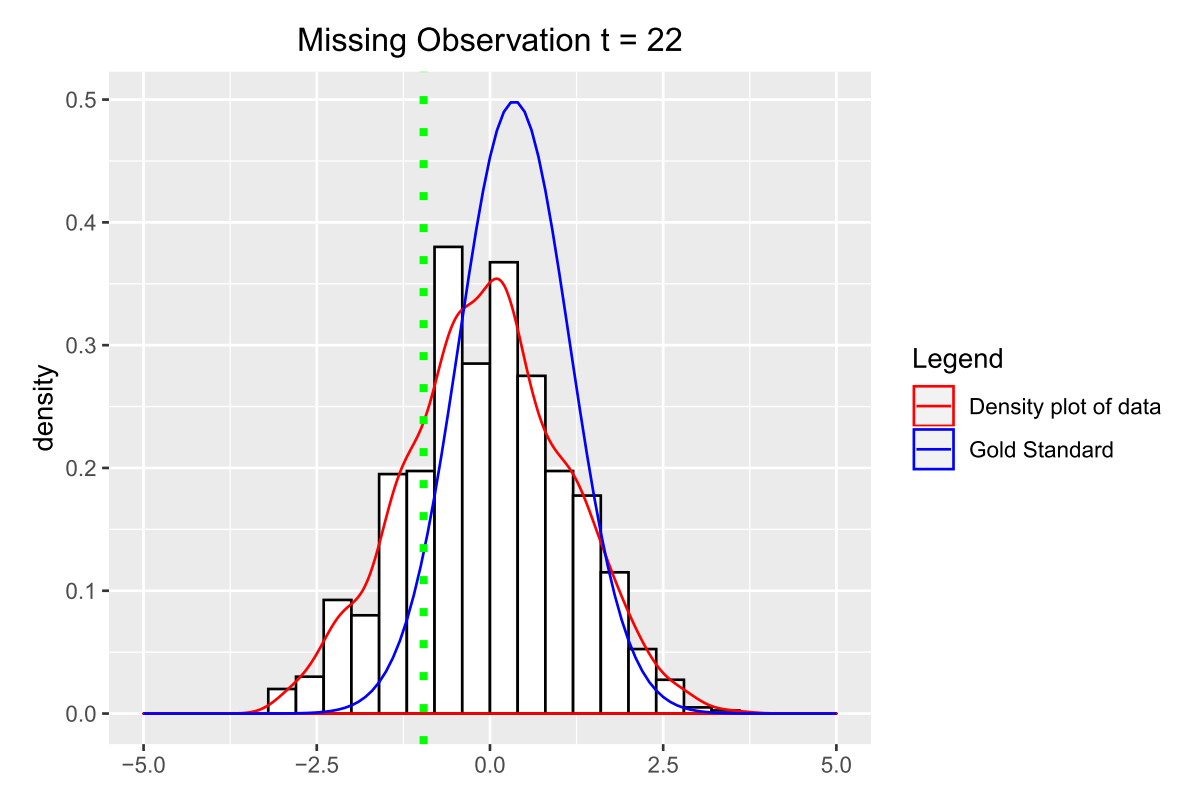
\includegraphics[width=0.3\linewidth]{Thesis/ar1_001.PNG}}
    \subfloat{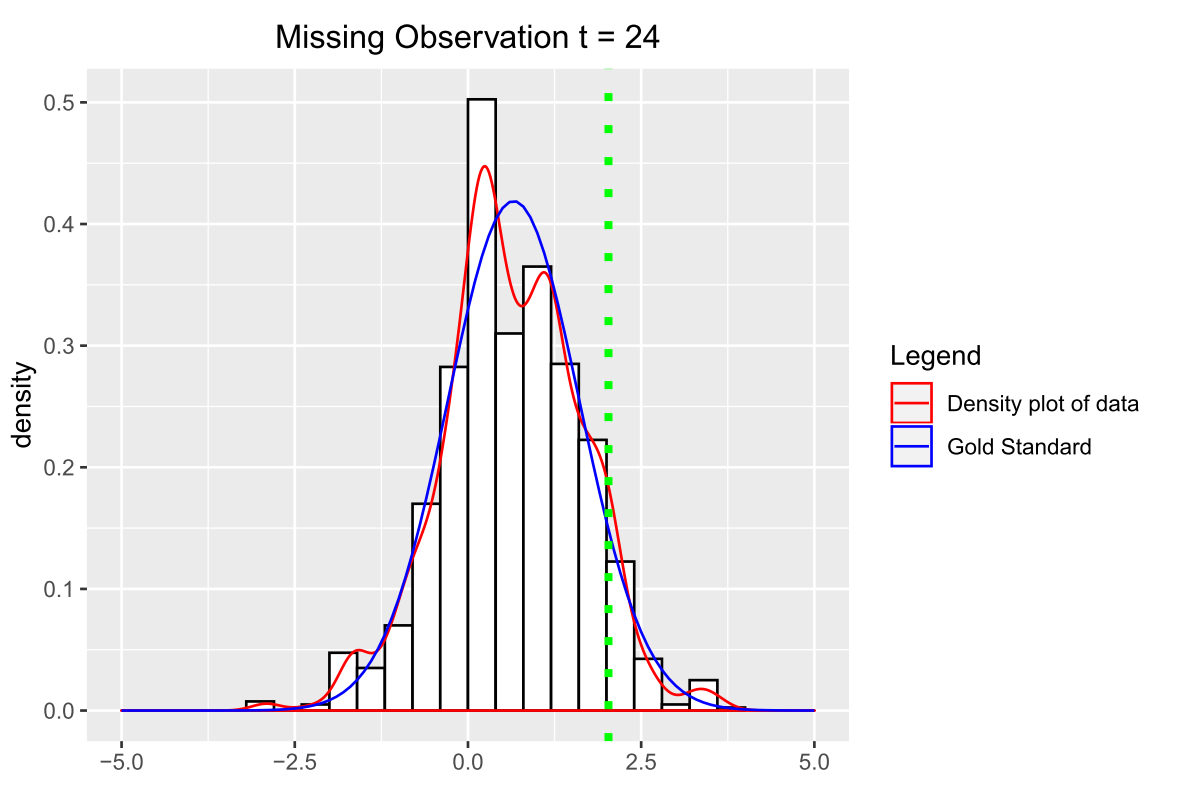
\includegraphics[width=0.3\linewidth]{Thesis/ar1_002.PNG}}\\
    \subfloat{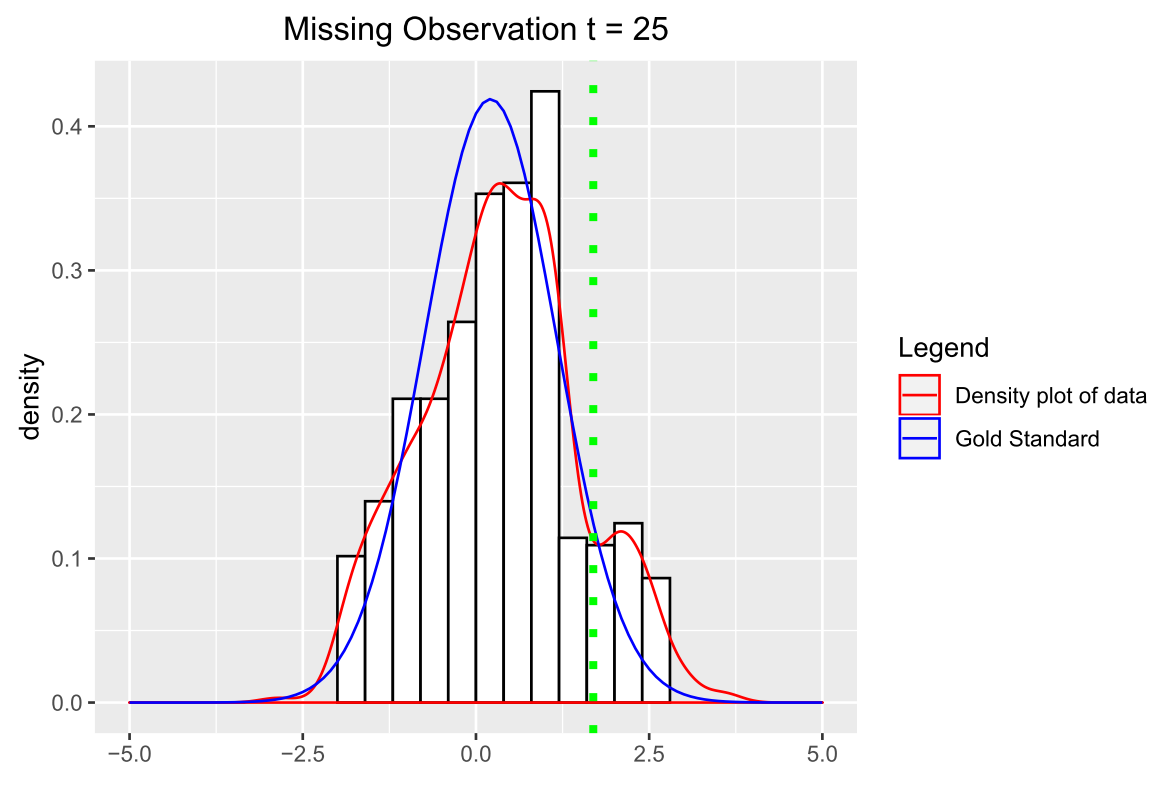
\includegraphics[width=0.3\linewidth]{Thesis/ar1_003.PNG}}
    \subfloat{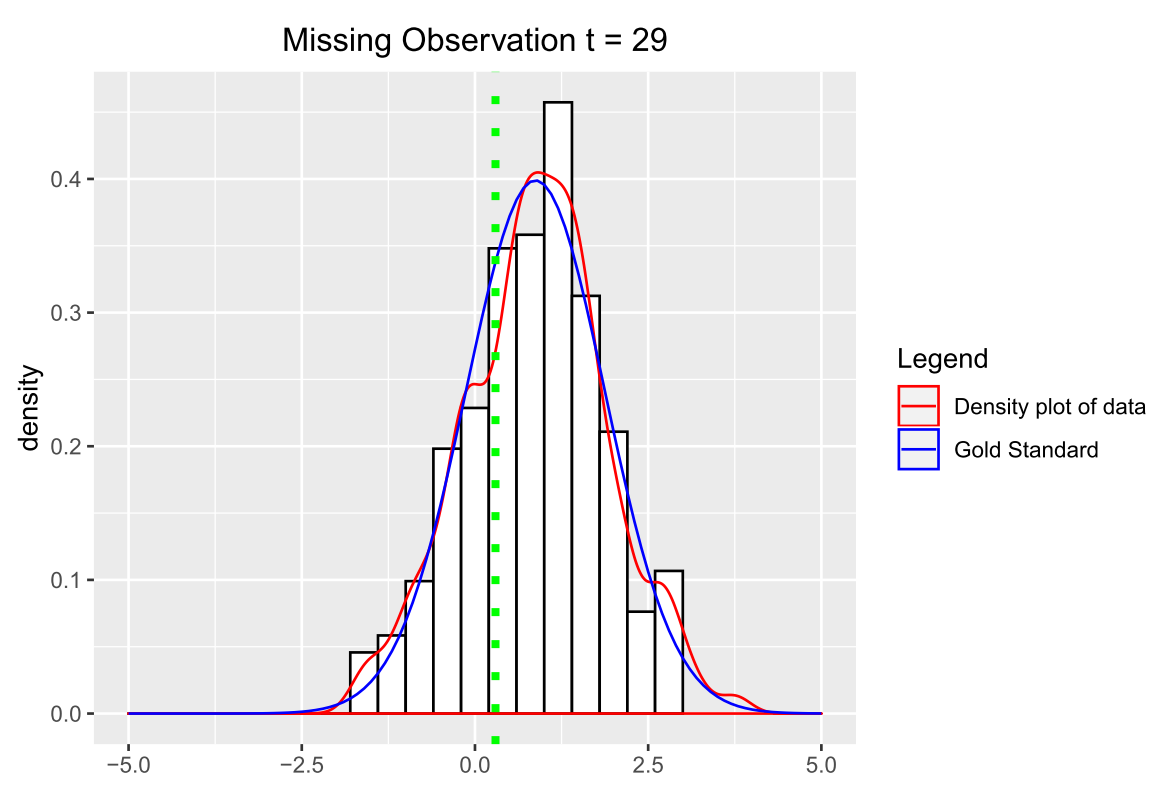
\includegraphics[width=0.3\linewidth]{Thesis/ar1_004.PNG}}
    \subfloat{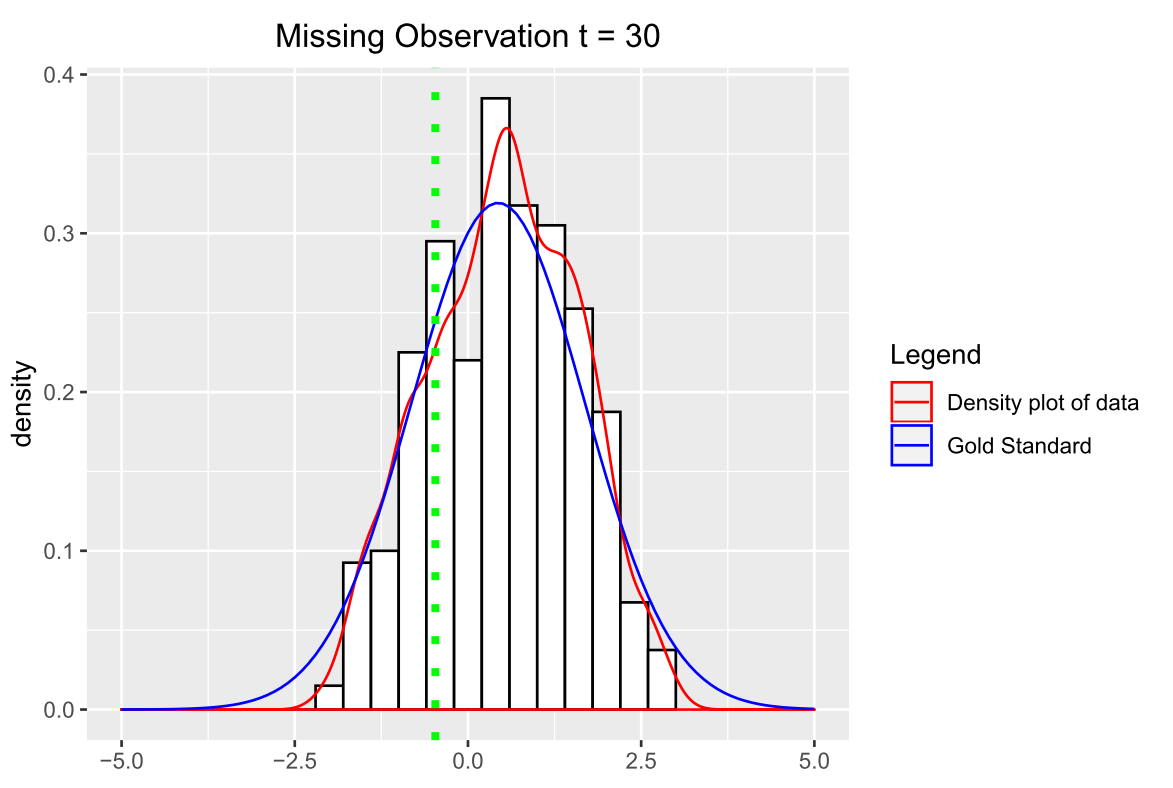
\includegraphics[width=0.3\linewidth]{Thesis/ar1_005.PNG}}
    \caption{AR(1) MODEL: Simulations with 1,000 particles and 30 times compared to the gold standard for the 5 missing times of the AR(1) model. In Green the value for the observation. The AR(1) model had parameter $\varphi = 0.5$, variance $\sigma^2 = 1$. The Bernoulli distribution had parameter $p = 0.2$}
\label{fig:1}
%\end{minipage}
\end{figure}
\end{frame}

\section{Application: A River Invasion}

\begin{frame}
\frametitle{A River Invasion}
    \begin{itemize}
        \item One-dimensional environment without tributaries or confluences. 
        \item The length of the river is divided into $N$ sections.
        \item The first introduction of the invasive species occurs in a cell with index $m$.
        \item The invasion can propagate only in the immediately adjacent sections of the river, (cells indexed by $m-1$ and $m+1$).
        \item At each time step, a cell becomes infested from an adjacent infested cell with probability $\theta$.
        \item Observations are made by a a probe that checks only the unobserved cells adjacent to cells where the invasive species has been detected.
        \item If that cell is both invaded and observed, adjacent cells will also be probed, and so on until a cell in which no invaders are detected is found.  The probability of observing invaders in an infested cell is denoted $\varphi$.
        \item The probe might fail to observe an invader that is present, and hence searching may stop without finding all invaded cells.
    \end{itemize}
\end{frame}

\begin{frame}
\frametitle{Application to the River Invasion}

Similarly to the AR(1) model, since our corrections are deterministic, the unnormalised weights are calculated as follows:
\begin{equation*}
    \frac{q(\bm{(X')}^{t}_i,\bm{(z')}^{t}_i | \bm{Z}^{t-1})}{q(\bm{X}^{t}_i,\bm{z}^{t}_i | \bm{Z}^{t-1})}
\end{equation*}

where the primed are the corrected terms and where
\begin{align*}
    & q(\bm{X}^{t},\bm{z}^{t} | \bm{Z}^{t-1}) =  \prod_{i=2}^{t} \varphi^{(a^{i} - a^{i-1})}\bigg(1 - \varphi \bigg)^{1-\one {a^i=\gamma^i}} \nonumber \\
    & \varphi^{(c^{i} - c^{i-1})} \bigg(1 - \varphi\bigg)^{1-\one {c^i=\beta^i}} \; \prod_{i=2}^{\min\{t,r\}} \theta^{k_i} (1-\theta)^{1-k_i}  \label{eq:4} \\ 
    & \prod_{i=2}^{\min\{t,l\}} \theta^{h_i} (1-\theta)^{1-h_i} \nonumber,
\end{align*}
and a there is a similar expression for the primed terms.

Here $l$ is the time at which the invasion has reached the left end of the modelled region, $r$ is the time at which the invasion has reached the right end of the modelled region, $k_i \in \{0,1\}$ and $h_i \in \{0,1\}$ where $k_i$ is 1 if the invasion expanded one cell to the right at time $i$ and $h_i$ is 1 if the invasion expanded one cell to the left at time $i$.

\end{frame}


\begin{frame}{Simulation of the river invasion}
    \begin{figure*}
        \begin{columns}
            \column{.3\linewidth}
            Simulation of 3 invasions with 1,000 particles and 50 cells all with $\theta = 0.3$. The left column shows the simulations while the left column shows the same simulations with observations superimposed in solid red. A1 and A2 show the invasion with $\varphi = 0.3$, B1 and B2 show the invasion with $\varphi = 0.1$. Figure C1 and C2 show the invasion with $\varphi = 0.8$.
            \label{fig:2}
            \column{.6\linewidth}
            %\includegraphics[width=\textwidth]{Thesis/river_007.png}
        \end{columns}
    \end{figure*}
\end{frame}


\section{Application: The RIFA invasion}

\begin{frame}
\frametitle{The RIFA invasion Model}
A key feature of our model is that it does not need to include the phylogeny of the nests in the likelihood, which should result in a much lower computational time when running the inference code. This will allow the model to be adapted to any type of problems where control strategies will have to be decided rapidly as new data is acquired. Notice that the phylogeny can can be reconstructed if needed. Also the new SIS method presents and efficient way to recalculate the weights as new observations arrive since it does not require to run again the entire code and many cancellations will occur during the calculation. 


\begin{itemize}
\item We need a model that can be fast and can be applied to point data as opposed to grid data.
\item This new model has the following features:
    \begin{itemize}
        \item Does not need to consider the phylogeny of the nests (faster), However, the phylogeny can be reconstructed if needed.
        \item Considers the detection process in parallel with the founding events.
        \item Includes unobserved nests alongside observed nests in the detection likelihood.
        \item Also, the application of the new `SIS with corrections' approach to this model presents and efficient way to recalculate the weights as new observations arrive since it does not require to run again the entire code.
    \end{itemize}
\end{itemize}
\end{frame}



\begin{frame}
\frametitle{RIFA Model: the intensity function}
    Here we consider a self-exciting spatial-temporal point process $N$ as a generalization of an Hawkes model \cite{Hawkes71}. We can then specify an intensity function $\lambda(x, y, t)$ which represents the infinitesimal expected  rate of events at time $t$ and location $(x, y)$.
    \begin{equation*}
        \lambda(x, y, t) = \mu(x, y, t) + \int_{0}^{t} \iint_{S} g(x - x', y - y', f - f') \d N(x', y', f')
    \end{equation*}
    where $\mu$ is the background term and $g$ is the clustering density.
\end{frame}

\begin{frame}
\frametitle{RIFA Model: the intensity function}
    We will consider the background to be zero, and we will consider the time and space elements of the clustering density to be independent.
    Also, the temporal behavior of the process is independent of the spatial behavior we can rewrite the conditional intensity as
    \begin{equation*}
        \lambda(x, y, f) = \int_{0}^{f} \iint_{S} r(f-f') l\Big((x - x'), (y - y')\Big) \d N(x', y', f')
    \end{equation*}
    where $m$ and $l$ are the triggering functions for time and space respectively.

    Since N is a counting measure, we can write this equation as

    \begin{equation*}
        \lambda(x, y, f) = \sum_{ p: f_p < f } r(f - f_p) l \Big((x - x_p),(y - y_p) \Big)
    \end{equation*}
    where the sum is over all the $p$ parent nests $(x_p, y_p, f_p)$ with $t_p < t$.
\end{frame}

\begin{frame}
\frametitle{RIFA Model: Maturation time}
    Each parent nest will be able to found more than one nest, with the number of nests founded per nest per month being a parameter $\zeta$, therefore the temporal triggering kernel will be a step function. Also the nests will have a maturation time $t_m$ of 8 months, meaning that before this time they will not be able to produce new nests. 

    The step function will be:

    \begin{equation*}
        r (f - f_p | \zeta) =
        \begin{cases}
            0, & \mbox{if} \quad f - f_p < t_{m} \\
            \zeta, & \mbox{if} \quad f - f_p \geq t_{m}
        \end{cases}
    \end{equation*}
    where $f$ is the founding time of the new nest and $f_p$ is the founding time of the parent nest.
\end{frame}


\begin{frame}
\frametitle{RIFA Model: Jumps}
    Biological invasions spread through local movements and by long-distance jumps \cite{Suarez}. We will therefore consider two unknown founding types: a local founding event with $U_i = 0$ and the long-distance jump with $U_i = 1$. The vector of jump type is therefore $U = (U_1, \dots, U_N)$ with $N$ the total number of founded nests.

    The vector of jumps types will have probability density function

    \begin{equation*}
        p(U| \gamma ) = {N \choose \nu}(\gamma)^{2\nu}(1 - \gamma)^{2(N - \nu)}
    \end{equation*}
    where $\gamma$ is the probability of a long jump and $\nu$ is the number of long-distance jumps.

    The  radial distance of the new nests from the parent nest will be distributed exponentially for the local founding event and with a L\'evy distribution for the long-distance jumps. The distribution over the angular direction will be uniform.
    Therefore the probability distributions for the short jumps $l_0$ and for the long jumps $l_1$ will be

    \begin{equation*}
        l_0\Big((x - x_p), (y - y_p) | U, \sigma \Big)= J \bigg(\frac{1}{2 \pi} \sigma e^{- \sigma r}\bigg)
    \end{equation*}

    \begin{equation*}
        l_1\Big((x - x_p), (y - y_p) | U, c \Big)= J \bigg(\frac{1}{2 \pi} \sqrt{\frac{c}{2 \pi}} \frac{e^{- \frac{c}{ 2 r}}}{r^{3/2}}\bigg)
    \end{equation*}
    where $J$ is the Jacobian and $r$ is the radial distance between the parents nests and the newly founded nests.
\end{frame}

\begin{frame}
\frametitle{RIFA Model: Nests Killed as Detected}
    We also make the assumption that nests are killed as soon as they are detected, so we introduce an indicator function $I(t_d - t)$ such that

    \begin{equation*}
        I (t_d - t) =
        \begin{cases}
            1, & \mbox{if} \quad t_d -  t> 0 \\
            0, & \mbox{otherwise}
        \end{cases}
    \end{equation*}
    where $t_d$ represents the time of detection. So the conditional intensity function will be

    \begin{equation*}
        \lambda(x, y, t, f) = \sum_{p:f_p < f} r(f - f_p | \zeta) I(t_d - t) p(U | \gamma) l_0(x, y | U, \sigma) l_1(x, y | U, c)
    \end{equation*}
    where we must have $f_p\leq t_d$.
\end{frame}

\begin{frame}
\frametitle{RIFA Model: Poisson Cluster Process}
    As demonstrated by Hawkes and Oakes \cite{Hawkes74}, any stationary self-exciting point process with finite intensity may be interpreted as a Poisson cluster process with the number of offspring for each event drawn from a Poisson distribution with mean 

    \begin{equation*}
        m = \int_0^T \iint_S g(x-x', y-y', f-f')\d N(x', y', f').
    \end{equation*}
    The likelihood, or joint pdf, at time $T$, will then be that of an inhomogeneous Poisson process for the founding process with intensity $\lambda(x, y, t)$
\end{frame}

\begin{frame}
\frametitle{RIFA Model: Detection Process}
    We will consider the detection processes in parallel with the founding events in a similar way as in Jewell's model for infectious diseases (\cite{Jewell}) : The time from establishment to notification $(t_i - f_i)$ of an offspring nest $i$ is a random variable exponentially distributed with parameter $\varphi$

    \begin{equation*}
    h(t_{i} - f_{i} | \varphi) = \varphi \exp (- \varphi(t_{i} - f_{i})).
    \end{equation*}
    
\end{frame}

\begin{frame}
\frametitle{RIFA Model: The Likelihood}
    The Likelihood for a set of $n$ locations $(s_{1}, ... , s_{n})$ with $s_i = (x_i, y_i)$, founding times $f_{1}, ... , f_{n}$, and detection times $(t_{1},  ... , t_{n})$ will then be:
    \begin{equation*} \label{eq:like}
        \begin{aligned}
            L = & \Bigg[ \prod_{i = 1}^{n} \lambda(s_{i}, t_{i}, f_{i}) \Bigg] \exp \Bigg(- \int_{0}^{T} \int_{0}^{T} \int_{S} \lambda(s, t, f) \d s \d t \d f \Bigg) \\ 
            & \prod_{\{ i : t_{i} < T \} } h(t_{i} - f_{i}) \prod_{ \{ i : t_{i} = \infty \} } \int_{T}^{\infty} h(t - f_{i}) \d t
        \end{aligned}
    \end{equation*}
    where $t_{i} = \infty$ if nest $i$ has not been detected at time $T$ and where $n$ is the number of nests founded. The quantity $h(t_{i} - f_{i})$ is the contribution of the observed nests, while $\int_{T}^{\infty} h(t - f_{i}) \d t$ is the contribution of the unobserved nest.
\end{frame}

\begin{frame}
\frametitle{RIFA Model: The Likelihood}
    Substituting the function $h$ and evaluating the last integral in equation above we get

    \begin{equation*}
        \begin{aligned}
            L = & \Bigg[ \prod_{i = 1}^{n} \lambda(s_{i}, t_{i}, f_{i}) \Bigg] \exp \bigg(- \zeta \sum_{i=1}^{n} (min\{ T, t_i \} - f_i) \bigg) \\ 
            & \prod_{\{ i : t_{i} < T \} } \varphi \exp (- \varphi (t_{i} - f_{i})) \prod_{ \{ i : t_{i} = \infty \} } \exp \bigg( - \varphi(T - f_{i}) \bigg).
        \end{aligned}
    \end{equation*}
    Notice that natural deaths are not considered in our model, so nests are immortal until detected and removed.
    
    This quantity will define the transition function $f(\bm{a}^{T_i} | \bm{A}^{T_{i-1}})$ of the system from one state to the next and will be the prior $q$ which represent the current state of the system. Notice that the model is Markovian, therefore each $\bm{a}^{T_i}$ is conditionally independent of $\bm{A}^{T_{i-2}} = (\bm{a}^{T_1}, \dots, \bm{a}^{T_{i-2}})$, given $\bm{a}^{T_{i-1}}$ and we will therefore have $f(\bm{a}^{T_i} | \bm{A}^{T_{i-1}}) = f(\bm{a}^{T_i} | \bm{a}^{T_{i-1}})$. 
\end{frame}



\begin{frame}
\frametitle{RIFA Model: The Corrections}
    Assume that each particle that has been simulated up to time $T_i$ can be corrected in a finite number of ways when we receive a new set of observations $\bm{z}^{T_i}$. We also make the assumption that a nests can be only corrected once and if corrected at time $T_j$ it will not be corrected again in future times. These corrections are made with probability $H_{z^{T_i}}((\bm{A}^{T_i})' | \bm{A}^{T_i})_{\zeta}$, where $(\bm{A}^{T_i})'$ is the vector of the corrected nests at time $T_i$.

    The probability $H_{z^{\tau_i}}((\bm{A}^{T_i})' | \bm{A}^{T_i})_{\zeta}$ of the new configuration of nests $\zeta$ will depend on the distances between the simulated nests and the observed nests in the following way. 
    
    Let us consider a simulated nest $a_j$ and an observation $z_h$. Then $a_j$ can be corrected by $z_h$ with probability $p_{a_j z_h} = p(a_j \leftrightarrow z_h) = e^{-d_{a_j z_h}}$ where $d_{a_j z_h}$ is the Euclidean distance between $a_j$ and $z_h$. Notice that when the distance is $d_{s_j z_h} = 0$ the probability $p_{s_j z_h}$ is 1 and the observation coincide with the simulated nest. The probability of a certain new configuration of nests will therefore be $H_{z^{T_i}}((\bm{A}^{T_i})' | \bm{A}^{T_i})_{\zeta} \propto (\prod_{h = 1}^{M^{T_i}} (p_{a_j z_h}))_{\zeta}$ and after normalization $H_{z^{T_i}}((\bm{A}^{T_i})' | \bm{A}^{T_i})_{\zeta} = (\prod_{h = 1}^{M^{T_i}} (p_{a_j z_h}))_{\zeta} / \sum_{\zeta} (\prod_{h = 1}^{M^{T_i}} (p_{a_j z_h}))_{\zeta} $ where the sum is over all the possible configurations. Each set of simulated particles that have not been corrected, can be corrected in only a finite number of ways to produce an element of the non-empty finite set $O_{\bm{z}^{T_i}} (\bm{A}^{T_i})$ that contains all the allowed corrections. The correction is made selecting an element $(\bm{A}^{T_i})'$ from the set $O_{\bm{z}^{T_i}} (\bm{A}^T)$ with probability $H_{z^{T_i}}((\bm{A}^{T_i})' | \bm{A}^{T_i})_{\zeta}$. Configurations of nests where the distances between observed and simulated nests are small will be more probable than the one where those distances are big.

    Let us call $s$ the number of simulated nests that we want to correct and $o$ the number of observed nests. The way we make the substitution is valid regardless of the values of $s$ and $o$ and the number of possible configurations is that obtained in ordered sampling without replacement. If we have more observed nests than simulated nests, we will correct all simulated nests and add all the remaining observed nests to the new configuration. Similarly if we have more simulated nests than observed one we will correct only the number of nests that we observe and leave the remaining nests to be corrected at a later stage.
    It follows that the number of possible configurations will be $\frac{s!}{(s-o)!}$ if $s > o$, $o!$ if $s = o$, and $\frac{o!}{(o-s)!}$ if $o < s$.

    Each time a nest is corrected its new location will correspond to the location of one of the observed nest and the time of observation will be corrected too with the observed one.
\end{frame}

\begin{frame}
\frametitle{RIFA Model: The weights}
    Using similar arguments to the one used for the models with discrete times we get the weights
    \begin{equation*}
        w^{T_i}_k \propto \frac{p^*(\bm{(A')}^{T_i}_k, \bm{A}^{T_i}_k | \bm{Z}^{T_i})} {q^*(\bm{(A')}^{T_i}_k, \bm{A}^{T_i}_k | \bm{Z}^{T_{i-1}})}
    \end{equation*}
    which with non deterministic corrections will become

    \begin{equation*}
        w^{T_i}_k \propto \frac{r(\bm{z}^{T_i}| \bm{Z}^{T_{i-1}}) q(\bm{(A')}^{T_i}_k | \bm{Z}^{T_{i-1}}) u(\bm{(A)}^{T_i}) H_{(z')^{T_i}} (\bm{A}^{T_i}_k | \bm{(A')}^{T_i}_k)}{q(\bm{A}^{T_i} | \bm{Z}^{T_{i-1}}) H_{z^{T_i}} (\bm{(A')}^{T_i}_k | \bm{A}^{T_i}_k)}.
    \end{equation*}
    The quantities $H_{(z')^{T_i}} (\bm{A}^{T_i}_k | \bm{(A')}^{T_T}_k)$ and $H_{z^{T_i}} (\bm{(A')}^{T_i}_k | \bm{A}^{T_i}_k)$ are identical at each step and will cancel out. Also $u(\cdot)$ and $r(\cdot)$ will cancel out after normalisation and the normalised weights will be

    \begin{equation*}
        W^{T_i}_k = \frac{q(\bm{(A')}^{T_i}_k | \bm{Z}^{T_{i-1}})}{q(\bm{A}^{T_i}_k | \bm{Z}^{T_{i-1}})} \Bigg( \sum_{s=1}^n \frac{q(\bm{A}^{T_i}_s | \bm{Z}^{T_{i-1}})}{q(\bm{(A')}^{T_i}_s | \bm{Z}^{T_{i-1}})} \Bigg).
    \end{equation*}
\end{frame}

\begin{frame}[shrink=15]
\frametitle{Bibliography}
\begin{thebibliography}{}

{\small \bibitem [\protect\citeauthoryear{Beer}{1990}]{Beer} 
Beer, T.: The Australian National Bushfire model project. Math Comput. Model. 13(12), 49-56 (1990)

\bibitem [\protect\citeauthoryear{Del Moral}{2014}]{Del Moral} 
Del Moral, P., Murraly, L.M.: Sequential Monte Carlo with Highly Informative Observations. Math Comput. Model. 13(12), 49-56 (1990)

\bibitem [\protect\citeauthoryear{Geweke}{1989}]{Geweke} 
Geweke, B.: Bayesian Inference in Econometric Models Using Monte Carlo Integration. Econometrica 57(6): 1317–1339 (1989).

\bibitem [\protect\citeauthoryear{Hawkes}{1971}]{Hawkes71} Hawkes, A. G.:Spectra of some self-exciting and mutually exciting point processes. Biometrika. 58(1): 83-90 (1971).

\bibitem [\protect\citeauthoryear{Hawkes and Oakes}{1974}]{Hawkes74} Hawkes, A. G., Oakes, D.: A cluster Process Representation Of A Self-Exciting Point Process. Journal of Applied Probabilities. 11(3): 493-503 (1974).

\bibitem [\protect\citeauthoryear{Jewell et al.}{2009}]{Jewell} Jewell, C. P., Kypraios, T., Neal, P.: Bayesian analysis for emerging infectious diseases. Bayesian Anal. 4(3): 465-496 (2009).

\bibitem [\protect\citeauthoryear{Keith}{2013}]{Keith} 
Keith J. M., Spring D.: Agent-based Bayesian approach to monitoring the progress of invasive species eradication programs. Pro.c Natl. Acad. Sci. 110(33): 13428-13433 (2013)

\bibitem [\protect\citeauthoryear{Malathy}{2011}]{Malathy} 
Malathy, A., Baboo, S.S.: An Enhanced Algorithm to Predict a Future Crime using Data Mining. Int. J. Comput. Appl. 21(1), 1-6 (2011)

\bibitem [\protect\citeauthoryear{Nakagawa}{2015}]{Nakagawa}
Nakagawa, S.: Missing data. In: Fox G.A., Negrete-Yankelevich S., Sosa V.J. (eds.) Ecological Statistics: Contemporary theory and application, pp 81-105. Oxford University Press (2015). 

\bibitem[\protect\citeauthoryear{O'Neill}{2002}]{O'Neill}
O'Neill, P.D., Roberts G.O.: Bayesian inference for partially observed stochastic epidemics. J. R. Stat. Soc. A. Stat. 162(1), 121-129 (2002)

\bibitem [\protect\citeauthoryear{Rubin}{1987}]{RubinMI}
Rubin, D.B.: Multiple imputation for nonresponse in surveys. Wiley, New York (1987)

\bibitem [\protect\citeauthoryear{Rubin}{1987}]{Rubin}
Rubin, D.B.: The Calculation of Posterior Distributions by Data Augmentation: Comment: A Noniterative Sampling/Importance Resampling Alternative to the Data Augmentation Algorithm for Creating a Few Imputations When Fractions of Missing Information Are Modest: The SIR Algorithm. J. Am. Stat. Assoc. 82(398), 543-546 (1987)

\bibitem [\protect\citeauthoryear{Rohlin}{1962}]{Rohlin}
Rohlin V.A.: On the fundamental ideas of measure theory.  Trans.
Amer. Math. Soc. 1(10): 1-52 (1962).

\bibitem [\protect\citeauthoryear{Suarez}{2000}]{Suarez} Suarez, A. V., Holway, A., Case, T. J.: Patterns of spread in biological invasions dominated by long-distance jump dispersal: Insights from Argentine ants. Proc Natl Acad Sci. 98(3): 1095-1100  (2000)

\bibitem [\protect\citeauthoryear{Tanner and Wong}{1987}]{Tanner}
Tanner, M.A., Wong, W.H.: The Calculation of Posterior Distributions by Data Augmentation. J. Am. Stat. Assoc. 82(398), 528-540 (1987)

\bibitem [\protect\citeauthoryear{Zhang}{2015}]{Zhang}
Zhang, X-P. et al.: Multiple Imputations Particle Filters: Convergence and Performance Analyses for Nonlinear State Estimation with Missing Data. IEEE J. Sel. Top Signa. 9(8), 1536-1547 (2015)}

\end{thebibliography}
\end{frame}






\end{document}
